% Title: gl2ps_renderer figure
% Creator: GL2PS 1.4.0, (C) 1999-2017 C. Geuzaine
% For: Octave
% CreationDate: Sun May 16 16:48:19 2021
\setlength{\unitlength}{1pt}
\begin{picture}(0,0)
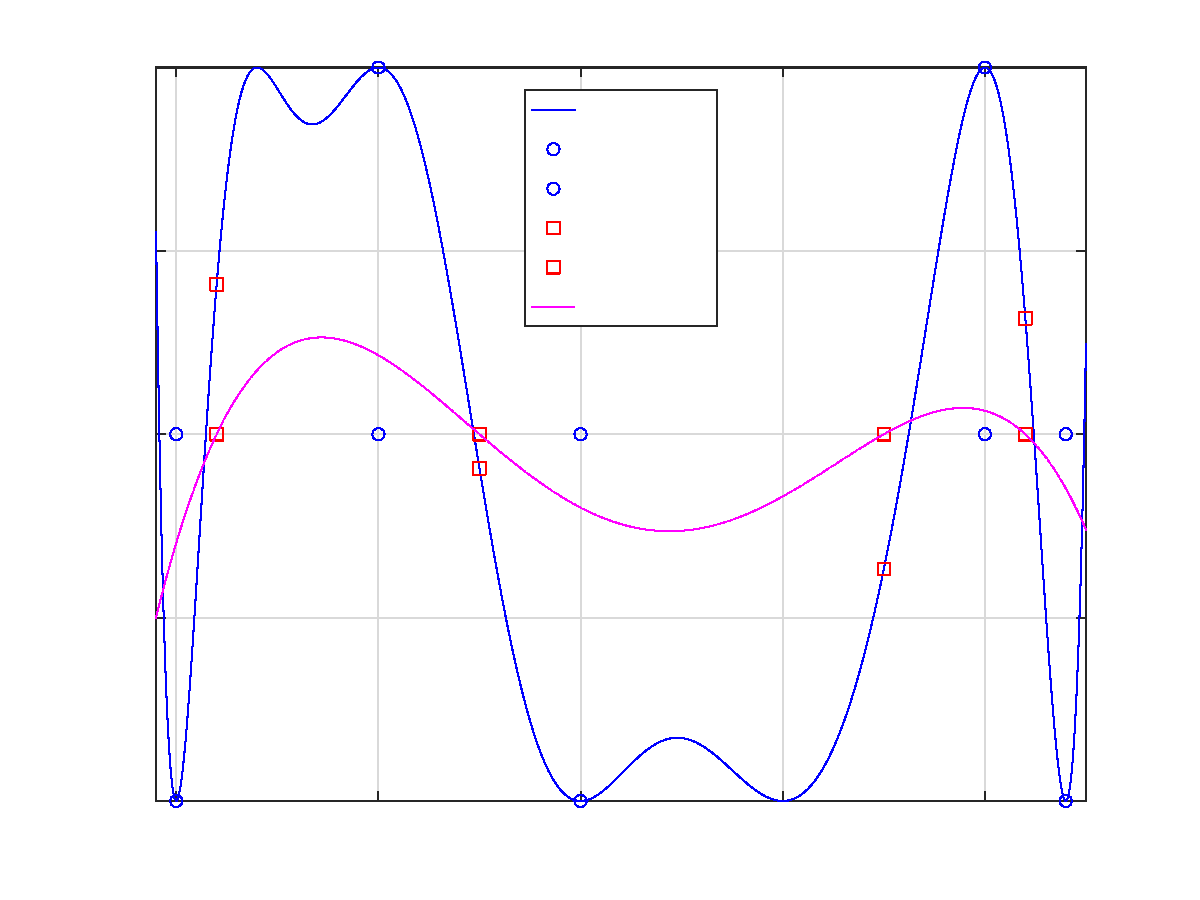
\includegraphics{figures/chap10/OUT/oscillation-inc}
\end{picture}%
\begin{picture}(576,432)(0,0)
\fontsize{10}{0}
\selectfont\put(84.5843,40.0183){\makebox(0,0)[t]{\textcolor[rgb]{0.15,0.15,0.15}{{0}}}}
\fontsize{10}{0}
\selectfont\put(181.628,40.0183){\makebox(0,0)[t]{\textcolor[rgb]{0.15,0.15,0.15}{{0.5}}}}
\fontsize{10}{0}
\selectfont\put(278.671,40.0183){\makebox(0,0)[t]{\textcolor[rgb]{0.15,0.15,0.15}{{1}}}}
\fontsize{10}{0}
\selectfont\put(375.715,40.0183){\makebox(0,0)[t]{\textcolor[rgb]{0.15,0.15,0.15}{{1.5}}}}
\fontsize{10}{0}
\selectfont\put(472.758,40.0183){\makebox(0,0)[t]{\textcolor[rgb]{0.15,0.15,0.15}{{2}}}}
\fontsize{10}{0}
\selectfont\put(69.8755,47.52){\makebox(0,0)[r]{\textcolor[rgb]{0.15,0.15,0.15}{{-1}}}}
\fontsize{10}{0}
\selectfont\put(69.8755,135.54){\makebox(0,0)[r]{\textcolor[rgb]{0.15,0.15,0.15}{{-0.5}}}}
\fontsize{10}{0}
\selectfont\put(69.8755,223.56){\makebox(0,0)[r]{\textcolor[rgb]{0.15,0.15,0.15}{{0}}}}
\fontsize{10}{0}
\selectfont\put(69.8755,311.58){\makebox(0,0)[r]{\textcolor[rgb]{0.15,0.15,0.15}{{0.5}}}}
\fontsize{10}{0}
\selectfont\put(69.8755,399.6){\makebox(0,0)[r]{\textcolor[rgb]{0.15,0.15,0.15}{{1}}}}
\fontsize{9}{0}
\selectfont\put(279.124,379.182){\makebox(0,0)[l]{\textcolor[rgb]{0,0,0}{{$(x,f(x)-p(x))$}}}}
\fontsize{9}{0}
\selectfont\put(279.124,360.318){\makebox(0,0)[l]{\textcolor[rgb]{0,0,0}{{$(x_i,f(x_i)-p(x_i))$}}}}
\fontsize{9}{0}
\selectfont\put(279.124,341.453){\makebox(0,0)[l]{\textcolor[rgb]{0,0,0}{{$x_i$}}}}
\fontsize{9}{0}
\selectfont\put(279.124,322.589){\makebox(0,0)[l]{\textcolor[rgb]{0,0,0}{{$(\xi_i,f(\xi_i)-p(\xi_i))$}}}}
\fontsize{9}{0}
\selectfont\put(279.124,303.725){\makebox(0,0)[l]{\textcolor[rgb]{0,0,0}{{$\xi_i$}}}}
\fontsize{9}{0}
\selectfont\put(279.124,284.86){\makebox(0,0)[l]{\textcolor[rgb]{0,0,0}{{$(x,s(x))$}}}}
\end{picture}
